
\section{Example: Modeling the Greenland ice sheet (EISMINT-Greenland)}\label{sec:eismint-greenland} \index{PISM!running the EISMINT-Greenland intercomparison}\index{Ice Sheets!Greenland ice sheet}\index{EISMINT!intercomparison of Greenland models} 
\optsection{EISMINT-Greenland}

In this section we give an extended example of how to use PISM to model the Greenland ice sheet.  We use older data from the 1990s ice sheet modelling intercomparison EISMINT-Greenland \cite{HuybrechtsEISMINT,RitzEISMINT}, but it is an excellent tutorial example.  The data are freely available at

\begin{center}
  \url{http://homepages.vub.ac.be/~phuybrec/eismint/greenland.html}
\end{center}

\noindent The snow-fall accumulation map, ablation parameterization, surface temperature formula, surface elevation, and bedrock elevation maps are essentially as in the 1991 papers \cite{Letreguillyetal1991,OhmuraReeh}.  In the ``forced climate'' CCL3 run, described below, the modeled ice sheet sees changes in surface temperature from the GRIP core \cite{Dansgaardetal1993} and sea level changes from SPECMAP \cite{Imbrieetal1984}.

Substantial developments have occurred in modeling the Greenland ice sheet since the EISMINT-Greenland intercomparison.  For example, the relation between a Greenland ice sheet flow model, Earth deformation under ice sheet loads, and the reconstruction of global ice loading is analyzed in \cite{TarasovPeltier}.  A parameter-sensitivity study of a EISMINT-Greenland-type ice sheet model is described in \cite{RitzFabreLetreguilly}.  The response of Greenland ice sheet models to climate warming is addressed in \cite{HuybrechtsdeWolde,Huybrechts02, Greve00}, among other references.

The rest of this section is a step-by-step PISM tutorial.  The details can be typed in by hand, or the user can invoke the bash scripts \texttt{preprocess.sh}, \texttt{bootstrap.sh}, \texttt{ssl2.sh}, and \texttt{ccl3.sh} in the directory \texttt{examples/eisgreen}.  These scripts execute the commands in the next four subsections, respectively.

\subsubsection*{Obtaining and pre-processing the EISMINT-Greenland data}  We use two Python scripts to convert the EISMINT-Greenland data.  The data is in the form of several ASCII text files, so we convert them into NetCDF files usable by PISM.  The Python libraries \href{http://numpy.scipy.org/}{\texttt{numpy}} and \href{http://code.google.com/p/netcdf4-python/}{\texttt{netcdf4-python}} must be present for the scripts to work.

First, \texttt{cd examples/eisgreen/} from the PISM directory, and download these text (ASCII) files from the EISMINT-Greenland web site above: 

\begin{verbatim}
grid20-EISMINT,  suaq20-EISMINT,  specmap.017,  sum89-92-ss09-50yr.stp
\end{verbatim}

\noindent (This is done by \texttt{preprocess.sh} using \texttt{wget}.) Once all four files have been downloaded, run

\begin{verbatim}
$ ./eisgreen.py
\end{verbatim}%$

\noindent The NetCDF file \texttt{eis_green20.nc} will be created from the data in \texttt{grid20-EISMINT} and \texttt{suaq20-EISMINT}.  It contains variables for the gridded latitude (\texttt{lat}), longitude (\texttt{lon}), surface altitude (``\texttt{usurf}'' for \textbf{u}pper \textbf{surf}ace elevation), ice thickness (\texttt{thk}), bedrock altitude (\texttt{topg}), and snow precipitation rate (\texttt{precip}; in ice-equivalent thickness units).  These values can be viewed graphically with \texttt{ncview}.  The metadata for these variables (the NetCDF ``header'') can be viewed by

\begin{verbatim}
ncdump -h eis_green20.nc
\end{verbatim}

The bed elevation \texttt{topg} in the original data (\texttt{suaq20-EISMINT}) effectively contains missing values.  These are locations where \texttt{topg} is \emph{exactly} $0.0$, presumably because in these locations the observed bed elevation was not measured or the measured value was not trusted.  We think these are deep fjords locations, mostly.  Also the topography of Ellesmere island is replaced by out of range negative values.  When viewing \texttt{eis_green20.nc} with \texttt{ncview}, these values show as white spots.  

If these missing values were to be left in the NetCDF handed to PISM then the resulting (very) rough bed elevation map would make reasonable ice flow results difficult.  We therefore smoothly fill the holes in the bed elevations.  This is done with another script named \texttt{fill_missing.py}\index{executables!python scripts!\texttt{fill_missing.py}}:\footnote{\texttt{fill_missing.py} is a general tool for smoothly filling patches of missing values in variables in NetCDF files.  It looks for attributes defining missing values and then fills in specified variables essentially by averaging the neighboring non-missing values.  It is found in directory \texttt{pism/util/}, it requires \href{http://code.google.com/p/netcdf4-python/}{\texttt{netcdf4-python}}, and it is documented in subsection \ref{subsect:scripts}.}:

\begin{verbatim}
$ fill_missing.py -f eis_green20.nc -v topg -o eis_green_smoothed.nc
\end{verbatim}%$

\begin{figure}[ht]
\centering
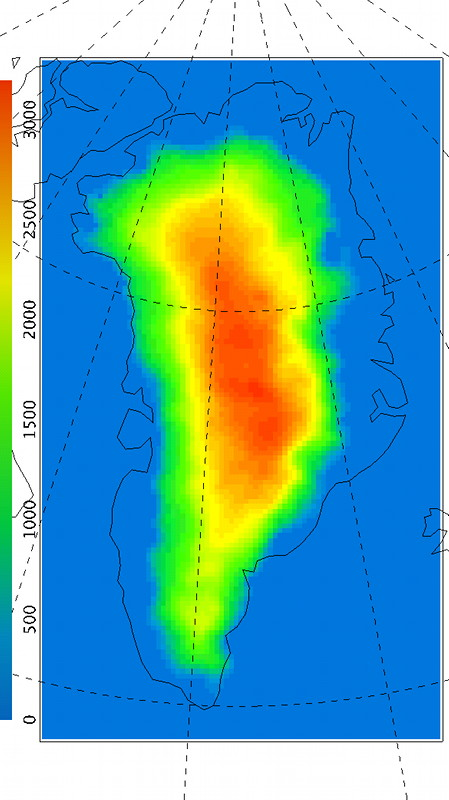
\includegraphics[width=2.4in,keepaspectratio=true]{EISgreen-thick}\quad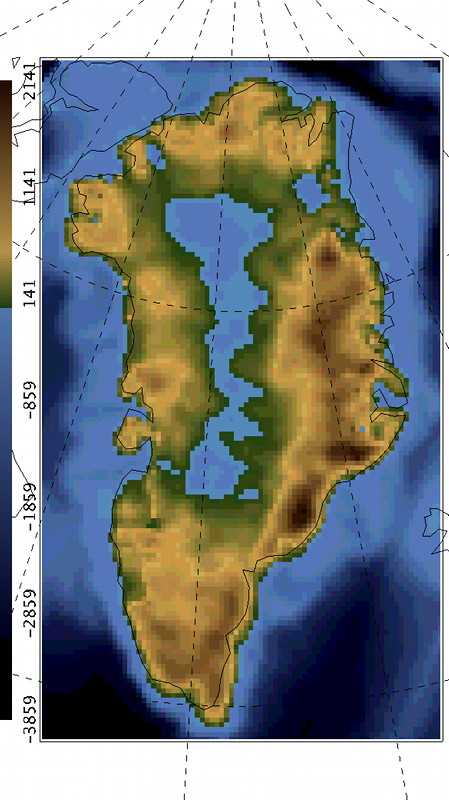
\includegraphics[width=2.4in,keepaspectratio=true]{EISgreen-bed}
\caption{Views of the thickness (left) and smoothed bed elevation (right) for EISMINT-Greenland.  The coastal topography around several fjords has been smoothed.}
\label{fig:greendata}
\end{figure}

Next we use a script which converts the time-series data files \texttt{specmap.017} and \texttt{sum89-92-ss09-50yr.stp} to PISM-readable NetCDF form:

\begin{verbatim}
$ ./eiscore.py
\end{verbatim}%$

\noindent Two NetCDF files with one-dimensional time series data are created, namely \texttt{grip_dT.nc} and \texttt{specmap_dSL.nc}.  In the paleoclimate run ``CCL3'' below, the executable \texttt{pismr} will be called with options \texttt{-dTforcing} and \texttt{-dSLforcing} on these two \texttt{.nc} files, respectively.  Thus PISM will read the GRIP data \cite{Dansgaardetal1993} for the surface temperature forcing and the SPECMAP data \cite{Imbrieetal1984} for sea level forcing.  Figure \ref{fig:gripDeltaT} shows the GRIP temperature offsets.

\begin{figure}[ht]
\centering
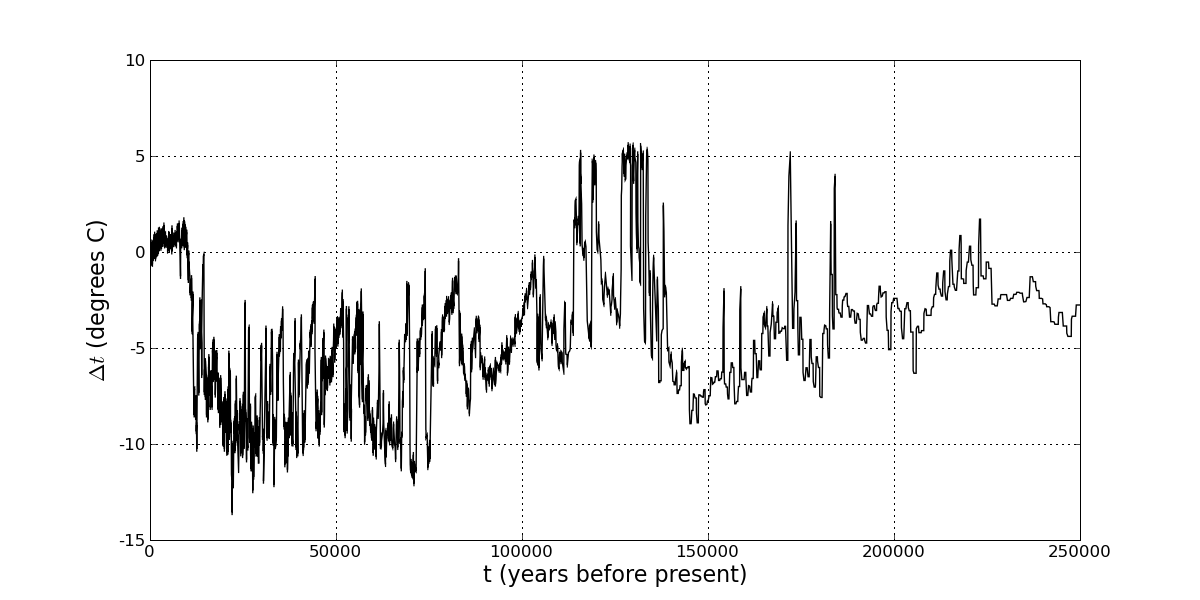
\includegraphics[width=5.6in,keepaspectratio=true]{gripDeltaT}
\caption{Change in temperature from present, from the GRIP core \cite{JohnsenetalGRIP}.}
\label{fig:gripDeltaT}
\end{figure}


\subsubsection*{Bootstrapping}  \label{sect:green-bootstrapping}  Once the EISMINT Greenland data is obtained and converted to NetCDF, as above, ``bootstrapping'' can begin.  By ``bootstrapping'' we mean the creation, by heuristics and simplified models, of the full initial conditions needed for the continuum model.  \footnote{The continuum model is the differential equations describing ice flow inside PISM.  See section \ref{sect:boot} for more on ``bootstrapping''.}

We do a one model year run using option \texttt{-boot_file} to ``bootstrap'' from file \texttt{eis_green_smoothed.nc}, using command-line options to enable an elevation- and latitude-dependent near-surface air temperature parameterization and a PDD model.

\begin{verbatim}
$ pismr -e 3 -ocean_kill -surface pdd -atmosphere eismint_greenland \
        -boot_file eis_green_smoothed.nc -Mx 83 -My 141 \
        -Lz 4000 -Mz 51 -Lbz 2000 -Mbz 21 -skip 1 -y 1 -o green20km_y1.nc
\end{verbatim}%$
\noindent The run takes only a few seconds of real time on any machine.  Tables \ref{bootstrapEISgreen} and \ref{bootCONTINUED} show the entire PISM output at the terminal.

\begin{table}
\centering
\scriptsize
\begin{quote}
\begin{verbatim}
PISMR trunk 0.4.1985 (basic evolution run mode)
  setting flow law to polythermal type ...
* Initializing bed smoother object with 5.000 km half-width ...
* Initializing the SIA stress balance modifier...
* Initializing Greenland atmosphere model based on the EISMINT Greenland (C. Ritz, 1997)
  air temperature parameterization and using stored time-independent precipitation...
    reading mean annual ice-equivalent precipitation rate 'precip'
      from eis_green_smoothed.nc ... 
  FOUND  precip    / mean annual ice-equivalent precipitation rate
                   \ min,max =     0.030,    2.820 (m year-1)
* Initializing the default temperature-index, PDD-based surface processes scheme.
  Precipitation and 2m air temperature provided by atmosphere are inputs.
  Surface mass balance and ice upper surface temperature are outputs.
  See PISM User's Manual for control of degree-day factors.
  Computing number of positive degree-days by: an expectation integral.
* Initializing the constant ocean model...
bootstrapping by PISM default method from file eis_green_smoothed.nc
  rescaling computational box for ice from -boot_file file and
    user options to dimensions:
    [-820.00 km, 820.00 km] x [-1400.00 km, 1400.00 km] x [0 m, 4000.00 m]
  WARNING: surface elevation 'usurf' found; IGNORING IT!
  reading 2D model state variables by regridding ...
  FOUND  lon       / standard_name=longitude 
                   \ min,max =   -94.194,   12.889 (degree_east)
  FOUND  lat       / standard_name=latitude  
                   \ min,max =    58.275,   84.458 (degree_north)
  FOUND  thk       / standard_name=land_ice_thickness
                   \ min,max =     0.000, 3200.000 (m)
  FOUND  topg      / standard_name=bedrock_altitude
                   \ min,max = -3859.000, 2151.000 (m)
  absent bwat      / effective thickness of subglacial melt water
                   \ not found; using default constant    0.00 (m)
  absent bmelt     / ice basal melt rate in ice thickness per time
                   \ not found; using default constant    0.00 (m year-1)
  FOUND  bheatflx  / upward geothermal flux at bedrock surface
                   \ min,max =    50.000,   50.000 (mW m-2)
  absent dbdt      / bedrock uplift rate
                   \ not found; using default constant    0.00 (m year-1)
  filling in ice and bedrock temperatures using surface temps and quartic guess
  ice enthalpy set from temperature, as cold ice (zero liquid fraction)
done reading eis_green_smoothed.nc; bootstrapping done
\end{verbatim}
\end{quote}
\normalsize
\bigskip
\caption{Output of bootstrapping command.  Continues in Table \ref{bootCONTINUED}.}
\label{bootstrapEISgreen}
\end{table}

\begin{table}
\centering
\scriptsize
\begin{quote}
\begin{verbatim}
* Initializing the bedrock thermal unit ... setting constants ...
  bootstrapping to fill lithosphere temperatures in bedrock thermal layers,
    using provided bedtoptemp and a linear function from provided geothermal flux ...
computational domain and grid:
                grid size   83 x 141 x 51
           spatial domain   1640.00 km x 2800.00 km x 4000.00 m
     horizontal grid cell   20.00 km x 20.00 km
  vertical spacing in ice   uneven, 51 levels, 21.200 m < dz < 138.800 m
   time interval (length)   [ 0.00 a, 1.00 a]  (1.0000 a)
* Using ice thickness at the beginning of the run
  to set the fixed calving front location.
doing preliminary step to fill diagnostic quantities ...
running forward ...
P         YEAR:     ivol     iarea     max_diff
U        years 10^6_km^3 10^6_km^2     m^2 s^-1
S      0.00000:  2.82500    1.6708   9.87263673
 $v$Eh d (dt=0.15391)
S      0.15391:  2.82512    2.2308   9.87263673
 $v$Eh d (dt=0.21700)
S      0.37091:  2.82525    2.1280   6.99952416
 $v$Eh d (dt=0.24986)
S      0.62077:  2.82491    1.6724   6.07770786
 $v$Eh d (dt=0.28176)
S      0.90253:  2.82503    1.7692   5.38835851
 $v$Eh e (dt=0.09747)
S      1.00000:  2.82510    2.2308   4.89872732
... done with run
Writing model state to file `green20km_y1.nc'
\end{verbatim}
\end{quote}
\normalsize
\bigskip

\caption{Continuation of Table \ref{bootstrapEISgreen}.}
\label{bootCONTINUED}
\end{table}

What has happened?  As noted, \emph{all} real ice sheet data fails to contain certain variables necessary to initialize an ice sheet model, in the sense of complete initial values for time-dependent partial differential equations.  For instance, the data and the observation-based parameterizations do not include the temperature of the ice anywhere but at the surface.  The data do not include the amount of water stored at the ice/bedrock interface.  And so on.  These are not omissions from the data sets but rather inevitable facts; one cannot observe ice sheets as fluids very well.  Necessarily, therefore, PISM fills in the unknown initial conditions based on some default guesses, as indicated by the messages in Table \ref{bootstrapEISgreen}.

Note that EISMINT-Greenland specifies an 83 by 141 point grid, but you may use other numbers for \texttt{-Mx} and \texttt{-My} if desired.  In such cases the data will be linearly interpolated onto your grid.  Larger values will produce slower runs.

The option \texttt{-boot_file} stands for ``bootstrap from file''.  A different option \texttt{-i}, for ``input file'', is used for a file which has full initial conditions.  In practice, \texttt{-i} is only used with a NetCDF file which was previously saved by PISM.  That is, \texttt{-i} is used to continue a run from a saved state.

Note the choice of the height of the computational box (``\texttt{-Lz 4000}''), of the number of vertical levels (``\texttt{-Mz 51}'' for levels in ice and ``\texttt{-Mbz 21}'' for levels in bedrock). The messages to standard out show that the vertical spacing is about 20 m near the base and more than 130 m at the top of the computational box where it matters less.

We see the report that bootstrapping has applied an interpolation scheme to the surface temperatures and geothermal fluxes to estimate preliminary temperatures within the ice.  It is based on a heuristic for the typical amount of downward flow in a column.  Thus bootstrapping quickly creates a temperature field at depth, but it is not a field in equilibrium with the flow.

The bootstrapping mode also fills in several default values.  For instance, the variables \texttt{bwat} (effective thickness of basal water), \texttt{tillphi} (till friction angle), and \texttt{dbdt} (bed uplift rate) were not found in the input file.   They would be present in a saved PISM model state and they are part of the ``full initial conditions'' referred to earlier)  Also, the data had redundant surface elevation values, in the sense that PISM uses the computation ``\texttt{usurf = topg + thk}'' of the surface elevation from the ice thickness and the bed elevation, and we are warned that the thickness and bedrock elevations are used and the surface elevations are ignored.

In addition to the default bootstrapping actions there are additional settings special to EISMINT-Greenland.  For instance, there is no EISMINT-Greenland gridded data set for surface temperature \cite{RitzEISMINT}.  Instead there is a formula (parameterization) which determines the temperature as a function of latitude and surface elevation.  The code behind \texttt{-atmosphere eismint_greenland} knows this formula and uses it.  Note that PDD factors use the PISM default values simply because the values from \cite{RitzEISMINT} are chosen to be the PISM default values.

As suggested a few paragraphs back, it is helpful to do a better job of filling in the temperatures within the ice.  One way to do this is to have the temperature field and velocity field co-evolve according to the thermomechanical flow model while holding the upper ice surface stationary.  This is effectively a continuation of ``bootstrapping''.  The result is to create a temperature field which is approximately stationary with respect to advection and conduction.  We create this temperature field by running for 25000 years with non-evolving surface.  The option \texttt{-no_mass} turns off the map-plane mass continuity scheme, and thus any evolution of the surface.  

\begin{verbatim}
$ mpiexec -n 2 pismr -e 3 -ocean_kill -atmosphere eismint_greenland -surface pdd \
          -i green20km_y1.nc -no_mass -y 25000 -o green20km_Tsteady.nc
\end{verbatim}%$
\noindent This last run takes less than half of a processor-hour.  Parallel processing is effective here, up to perhaps a peak real time speed with 40 processors for this coarse 83$\times$141 grid.  (Finer grid computations, for instance on a 5km grid for a Greenland-sized ice sheet, are \emph{easier} to parallelize in the sense that greater maximum speedup over one processor is attainable \cite{BBssasliding}.)

The velocity field in \texttt{green20km_Tsteady.nc}, with which the temperature field is approximately in balance, is not one for which the surface kinematical equation \cite{Fowler}, equivalently the mass continuity equation, is satisfied.  So the temperature field is only approximately steady, and significant evolution resumes when we again ``turn on'' the mass continuity equation, as we do next.  Also, a longer run like the above would be reasonable because the exponential time constant for decay of the thermomechanically-coupled system toward equilibrium is on the order of 100k years, but the goal is merely to get to a state which is reasonable, before starting a complete steady-state run, as we are about to do.

The EISMINT-Greenland experiments \cite{RitzEISMINT} specify a positive degree day (PDD) model which is turned on using the \texttt{-surface pdd} option.  The PDD model is, by default, implemented by the deterministic scheme described in \cite{CalovGreve05}, but the user can add option \texttt{-pdd_rand} to use a stochastic PDD implementation.

\subsubsection*{Running the EISMINT-Greenland steady state experiments}  Now that we have initial conditions including a vaguely-credible temperature field and essentially the present day geometry (thickness), our first experiment is the steady state run ``SSL2'' turned on using the option \intextoption{ssl2}.  This experiment uses the parameters specified in the EISMINT-Greenland description \cite{RitzEISMINT}.  If 8 processors are used, a ten thousand model year run might look like this:

\begin{verbatim}
$ mpiexec -n 8 pismr -e 3 -ocean_kill -surface pdd -atmosphere eismint_greenland \
          -i green20km_Tsteady.nc -y 10000 -ys 0 -o green_SSL2_10k.nc
\end{verbatim}%$
\noindent We could continue for another ten thousand years by starting from the saved file and continuing for 10000 more model years:
\begin{verbatim}
$ mpiexec -n 8 pismr -e 3 -ocean_kill -surface pdd -atmosphere eismint_greenland \
          -i green_SSL2_10k.nc -y 10000 -o green_SSL2_20k.nc
\end{verbatim}%$
\noindent And so on.

The script \texttt{ssh2.sh} uses options \texttt{ts_file} and \texttt{extra_file} to save scalar and map-plane diagnostic quantities every year and every 1000 years, respectively. So our discussion will now assume that the user \emph{actually} did this to completion:

\begin{verbatim}
./ssl2.sh 2 >> out.ssl2 &
\end{verbatim}

\noindent This puts a two processor run in the background and generates a text file logging the whole run.  It should take something like 120 processor hours.  Three files appear, \texttt{vol_ssl2.nc}, \texttt{ex_ssl2.nc}, and, at the end of the run, \texttt{green_ssl2_110ka.nc}.

The SSL2 simulation is intended to go until the model reaches a ``steady state'', a phrase which \cite{RitzEISMINT} defines as a small volume change rate, namely less than a .01\% change in volume in 10,000 years.  One may see the behaviour over time of the volume, area, basal melt fraction, and a couple of other default quantities, by viewing the NetCDF file \texttt{vol_ssl2.nc}.  We leave it as an exercise to find the first 10000 model year period in which the volume changes by less that 0.01\%.

The volume shows a consistent growing-but-leveling-out trend, with a final volume a bit more than $4 \times 10^{6}\,\text{km}^3$.  The time series for volume and melt fraction (the fraction of the base where the temperature is at pressure-melting) are shown in Figures \ref{fig:eisgrnvolseries} and \ref{fig:eisgrnmeltfseries}.  The melt fraction indicates that, measured by basal melt fraction, the temperature field from bootstrapping and relaxing the temperature field (above) gave a pretty good estimate of the basal melt fraction for the fully-coupled steady state.

\begin{figure}[ht]
\centering
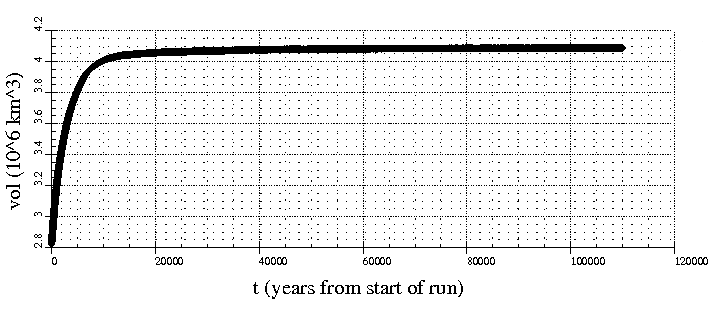
\includegraphics[width=6.0in,keepaspectratio=true]{eisgrn-volseries}
\caption{Volume time series for a 110k model year EISMINT-Greenland SSL2 run; units of $10^{6}\,\text{km}^3$.}
\label{fig:eisgrnvolseries}
\end{figure}

\begin{figure}[ht]
\centering
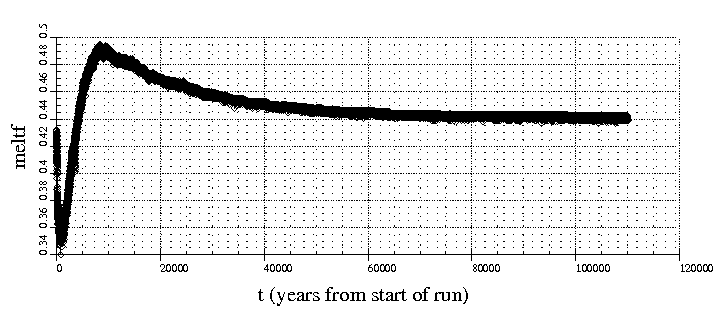
\includegraphics[width=6.0in,keepaspectratio=true]{eisgrn-meltfseries}
\caption{Time series for the fraction of the base which is at the pressure-melting temperature from a 110k model year EISMINT-Greenland run.  See the right hand part of Figure \ref{fig:ssl2thickTpa} for a map of the basal temperature.}
\label{fig:eisgrnmeltfseries}
\end{figure}

We will use the final NetCDF file \texttt{green_ssl2_110ka.nc} to continue the EISMINT-Greenland experiments below.  The saved ice thickness, basal temperature, and vertically-averaged horizontal velocity maps are shown in Figure \ref{fig:ssl2thickTpa}.

\begin{figure}[ht]
\centering
\mbox{\phantom{|}\hspace{-1.0in}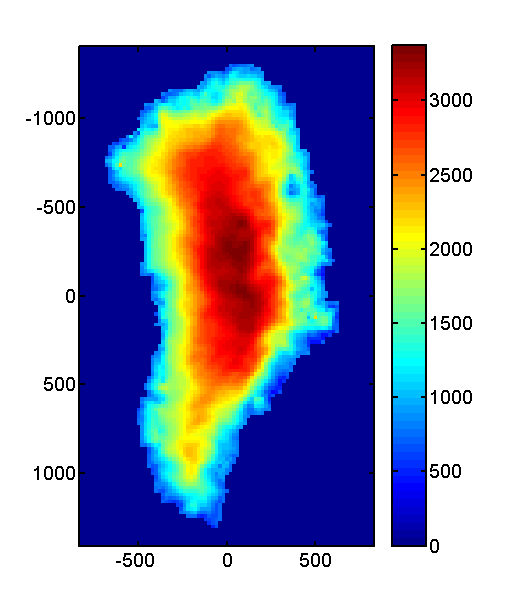
\includegraphics[height=3.0in,keepaspectratio=true]{greenH-SSL2}\,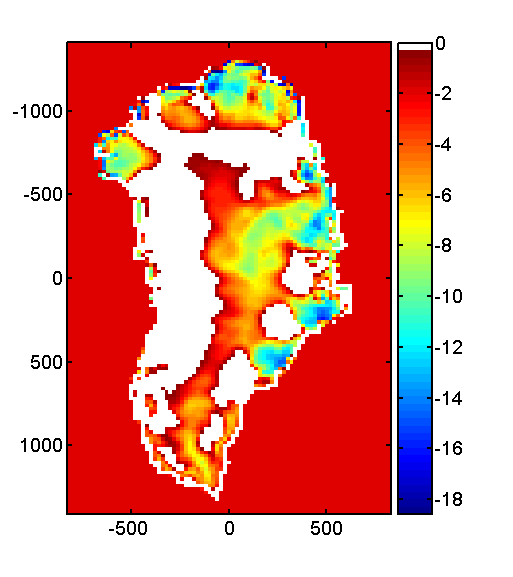
\includegraphics[height=3.0in,width=2.3in]{greenTpa-SSL2}\,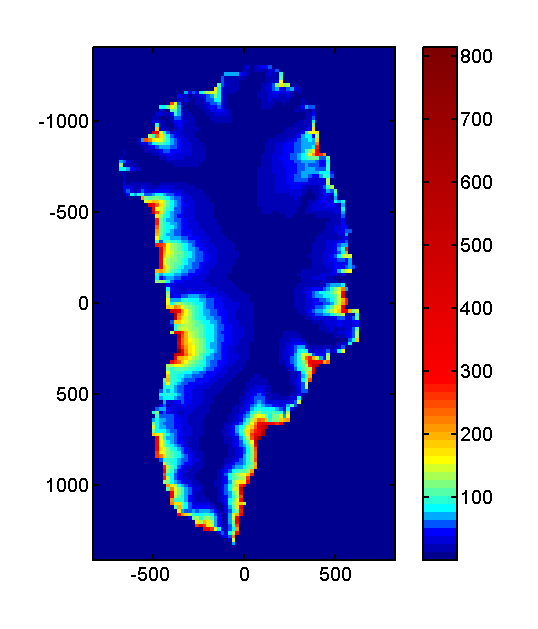
\includegraphics[height=3.0in,keepaspectratio=true]{greencbar-SSL2}}
\caption{Ice thickness (meters; left), basal temperature (degrees C below 0; middle), and vertically-averaged horizontal velocity (m/a; right) at the end (110k model years) of a EISMINT-Greenland SSL2 run.  Pressure-melting temperature areas are white.}
\label{fig:ssl2thickTpa}
\end{figure}

In addition to the standard EISMINT-Greenland intercomparison called ``SSL2'', a ``SSL3'' was proposed to allow each participant to choose additional parameters and adjust other aspects of the model.  (Sliding, for instance, is an outstanding omission here.)  We omit this for tutorial purposes, however, and proceed to use climate forcing in runs ``CCL3'' and ``GWL3''.


\subsubsection*{Climate forcing from GRIP and SPECMAP} 
\label{sec:climate-forcing}
The next experiment starts from the end of the steady state SSL2 run above.  Recall that the NetCDF files \texttt{grip_dT.nc} and \texttt{specmap_dSL.nc} contain time series data for change in surface temperature and sea level.  The options \texttt{-dTforcing} and \texttt{-dSLforcing} include these data for a ``CCL3'' climate forced run \cite{RitzEISMINT,HuybrechtsEISMINT}.  Before every time step, \texttt{pismr} reads the change to the surface temperature and sea level for that time.  The data in \texttt{grip_dT.nc} extends 250,000 years into the past, while the data in \texttt{specmap_dSL.nc} goes back about 780,000 years, so EISMINT-Greenland specifies that the run will start at the beginning of the GRIP data.  

The script \texttt{ccl3.sh} runs the CCL3 experiment for the full 250ka period, with this single command
\begin{verbatim}
mpiexec -n 8 pismr -e 3 -ocean_kill -bed_def lc
        -surface pdd -skip 10 -i green_ssl2_110ka.nc \
        -ys -249900 -ye 0 -atmosphere eismint_greenland,dTforcing \
        -dTforcing grip_dT.nc -ocean constant,dSLforcing \
        -dSLforcing specmap_dSL.nc -save_file snaps_ccl3.nc \
        -save_times -240000:10000:-10000 -ts_file vol_ccl3.nc \
        -ts_vars ivol -ts_times -249900:100:0 -o green_ccl3_year0.nc
\end{verbatim}
\noindent We turn on the Lingle and Clark \cite{BLKfastearth,LingleClark} two layer, flat earth bed deformation model, with an assumption of zero uplift rate at the start of the run, using option \intextoption{bed_def} \texttt{lc}.

The resulting thickness difference, relative to the end of the SSL2 run, and the pressure-adjusted basal temperature, are shown in Figure \ref{fig:cclthickTpa}.

\begin{figure}[ht]
\centering
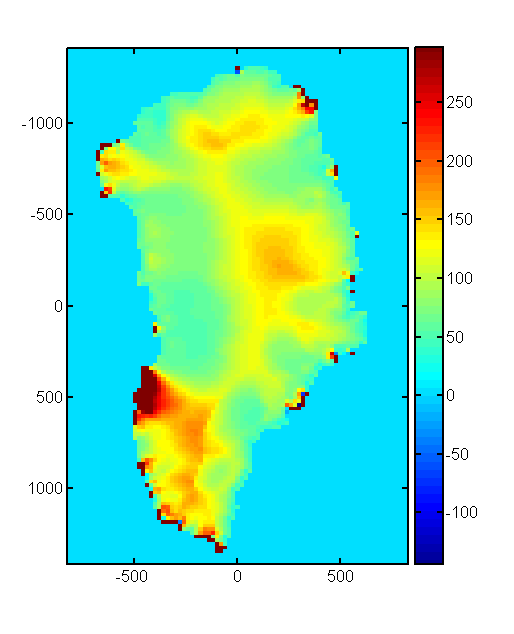
\includegraphics[width=2.8in]{Hdiff-CCLSSL}\quad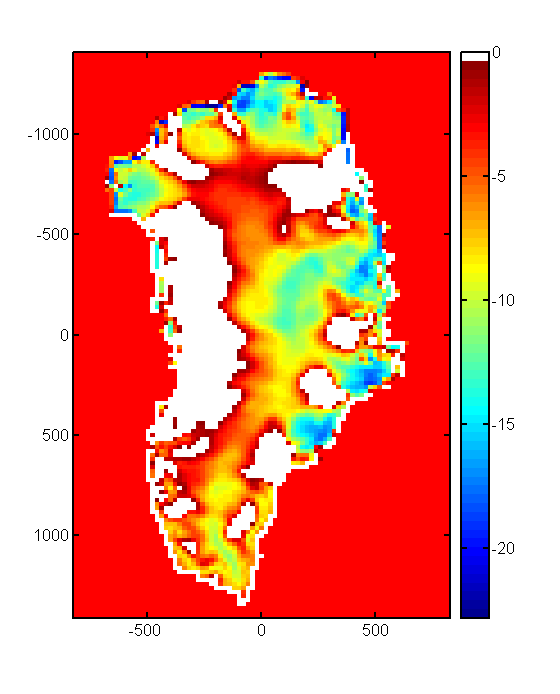
\includegraphics[width=2.8in]{Tpa-CCL}
\caption{Left:  Ice thickness difference between end (year zero) of a CCL3 run and the end of an SSL2 run (meters).  Right:  Ice pressure-adjusted basal temperature (degrees C below 0; right) at the end of a EISMINT-Greenland CCL3 run.  Compare Figure \ref{fig:ssl2thickTpa}.}
\label{fig:cclthickTpa}
\end{figure}

EISMINT-Greenland also calls for a baseline run for another 500 years which starts from the end of the CCL3 run and has steady current climate forcing (noting no GRIP or SPECMAP data are known from the future!):

\begin{verbatim}
mpiexec -n 8 pismr -e 3 -ocean_kill -bed_def lc \
        -surface pdd -atmosphere eismint_greenland \
        -i green_ccl3_year0.nc -y 500 -o green_ccl3_year500.nc
\end{verbatim}

A final ``greenhouse warming'' experiment ``GWL3'', turned on using \intextoption{gwl3_start_year}, is described in the EISMINT-Greenland \cite{RitzEISMINT}.  It runs for 500 years with the temperature increasing by $0.035^\circ C/$year for the first 80 years, then at a rate of $0.0017^\circ C/$year for the last 420 years:

\begin{verbatim}
mpiexec -n 8 pismr -e 3 -ocean_kill -bed_def lc \
        -surface pdd -atmosphere eismint_greenland \
        -gwl3_start_year 0 -i green_ccl3_year0.nc -y 500 -o green_gwl3_year500.nc
\end{verbatim}

\subsubsection*{Visualizing the climate inputs in the Greenland case}
\label{sec:pdd-series-with-pclimate}

Assuming that \texttt{green20km_y1.nc} was produced by the run above (see section
\ref{sect:green-bootstrapping}), one can run the following to check if the PDD
model in PISM (see section \ref{sec:boundary-models}) is ``reasonable'':
\begin{verbatim}
$ pclimate -i green20km_y1.nc -atmosphere eismint_greenland -surface pdd \
           -times 0.0:0.1:2.5 -o pddmovie.nc 
\end{verbatim}%$
This produces the file \texttt{pddmovie.nc} with several variables: \texttt{acab}
(instantaneous net ice equivalent accumulation (ablation) rate), \texttt{artm}
(mean annual temperature at ice surface but below firn), \texttt{airtemp}
(instantaneous near-surface air temperature), \texttt{precip} (mean annual
ice-equivalent precipitation rate) and some others.

Variables \texttt{artm} and \texttt{precip} do not evolve over time because the 
former is generated from ice sheet geometry and latitude by the EISMINT-Greenland formulas \cite{RitzEISMINT}, while the latter is part of the EISMINT-Greenland data itself.

The other two variables were used to create figure \ref{fig:pddseries}, which
shows the time-series of the accumulation rate (top graph) and the air
temperature (bottom graph) with the map view of the air temperature at time 0
over it. The cross on the latter shows (approximately) the location of the
point used for the time-series.

Here are two things to notice:
\begin{enumerate}
\item The summer peak day is in the right place.  The default for this value is
  August 1 (day $243$, at approximately $243/365 \simeq 0.66$ year).  (If it is
  important, the peak day can be changed using the \texttt{-pdd_summer_peak_day}
  option; subsection \ref{sec:boundary-models}).

\item Lows of the surface mass balance rate \texttt{acab} correspond to 
  positive degree-days in the given period, because of highs of the air
  temperature.  Recall the air temperature graph does
  not show random daily variations.  Even though it has the maximum of about $266$
  Kelvin, the parameterized instantaneous air temperature can be above freezing.
  A positive value for positive degree-days is expected \cite{CalovGreve05}.
\end{enumerate}

\begin{figure}[ht]
  \centering
  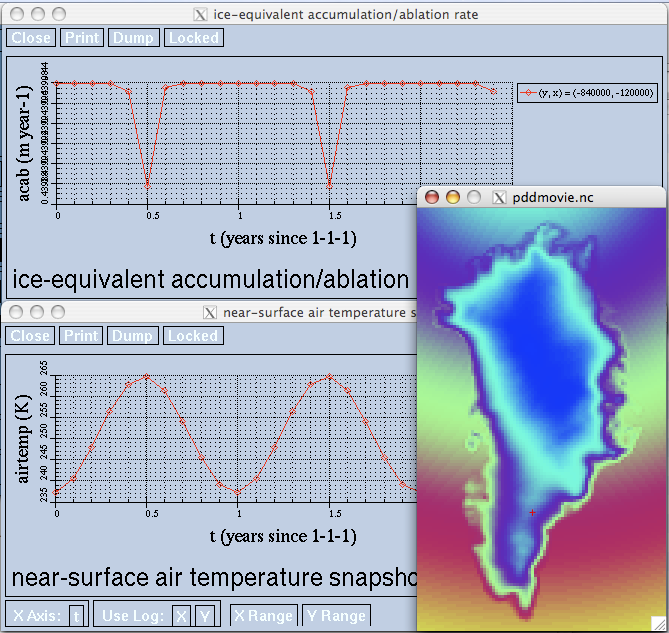
\includegraphics[width=5in]{pdd-timeseries}
  \caption{Time series of the surface mass balance rate and near-surface air temperature. Map view 
           on the right shows the location chosen.}
  \label{fig:pddseries}
\end{figure}

\bigskip
We can also test the surface temperature forcing code with the following command.
\begin{verbatim}
$ pclimate -i green20km_y1.nc -o dT_movie.nc \
           -atmosphere eismint_greenland,dTforcing -dTforcing grip_dT.nc \
           -times -2.5e5:2000:0
\end{verbatim}%$
The output \texttt{dT_movie.nc} and \texttt{grip_dT.nc} mentioned in section above were used to create figure \ref{fig:artm-timeseries}.

This figure shows the GRIP temperature offsets (top graph; compare to figure \ref{fig:gripDeltaT}) and the time-series of the temperature at the ice surface at a point in southern Greenland (bottom graph), confirming that the temperature offsets are used correctly.

\begin{figure}[ht]
  \centering
  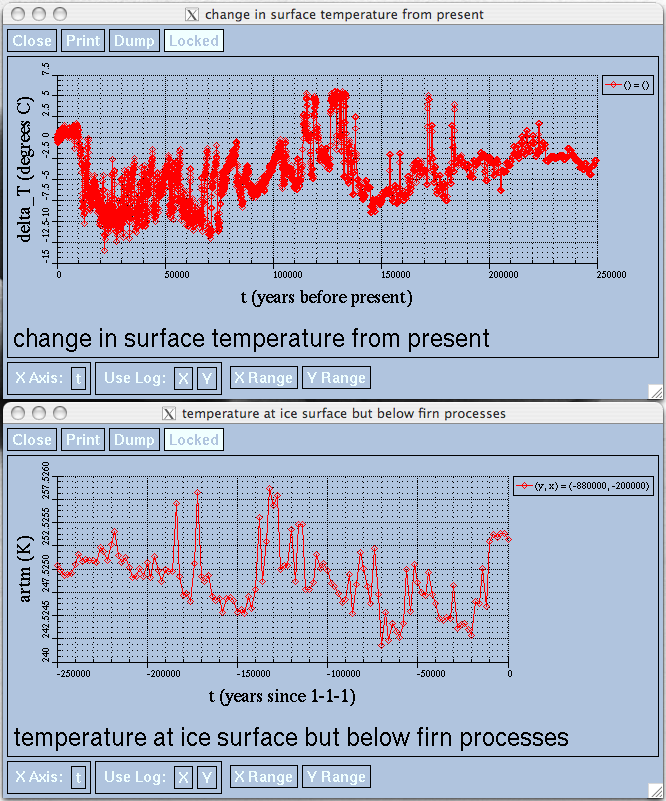
\includegraphics[width=5in]{artm-timeseries}
  \caption{Time series of the surface temperature compared to GRIP temperature offsets}
  \label{fig:artm-timeseries}
\end{figure}

\begin{comment}
  FIXME: Variable acab in following is worth looking at. It looks right and it
  may be possible to compare to other paleo-climate studies:
\begin{verbatim}
$ pclimate -i green20km_y1.nc -o bar.nc -times -125000.0:1000.0:0.0 \
           -dTforcing grip_dT.nc -dSLforcing specmap_dSL.nc \
           -atmosphere eismint_greenland,dTforcing -surface pdd -ocean constant,dSLforcing
\end{verbatim}%$
\end{comment}

%%% Local Variables: 
%%% mode: latex
%%% TeX-master: "manual"
%%% End: 

% LocalWords:  parameterized
